%%=============================
%% Appendix: Lax Representation
%%=============================

\documentclass[../dissertation.tex]{subfiles}

\begin{document}

The observant reader may notice that our choice of Lax pair for the ILW differs 
from Lax pair typically given in the literature. Indeed, the Lax Pair for the ILW
given in \cite{SATSUMA1979} and \cite{Kodama1982} is as follows:
\begin{subequations}
	\label{eq:ILW.lax}
	\begin{align}
		\label{eq:ILW.lax.x} 
		\frac{1}{i} \frac{\bd}{\bd x} \psi^+ + \mu_1\psi^+ + \mu_2\psi^- &= u \psi^+  \\
		\label{eq:ILW.lax.t}
		\frac{1}{i} \frac{\bd}{\bd t} \psi_t^\pm - 2i (\mu_1 + 1/2\delta) \psi_x^\pm - \psi_{xx}^\pm 
			&= \left[ \mp i u_x - T u_x + \nu \right]\psi^\pm,
	\end{align}
\end{subequations}
where, in our notation, $\mu_1$ and $\mu_2$ are given in terms of the 
the spectral parameter $\lambda$ as
\begin{align*} \label{LambdaAndMu}
	\mu_1 = - \frac{1}{2} \lambda \coth(\lambda \delta) \qquad \text{and} \qquad
	\mu_2 = \frac{1}{2}\lambda \csch(\lambda \delta),
\end{align*}
and $\nu$ is an arbitrary constant.

In order to see how the above Lax pair from the liturature compares with 
\eqref{eq0:Lax},
we consider the function $\psi$ 
as a function defined along the line $L:= \{z \in \CC \,:\, \im z = \delta\}$ 
whose analytic extension to the complex strip 
$\mc S := \{ z \in \CC \,:\,  0 < \im z < 2 \delta\}$
has boundary values $\psi^\pm$. That is, if $\Psi$ denotes the analytic
extension of $\psi$ to $\mc S$, then we define $\psi(x) := \Psi(x + i \delta)$
($x \in \RR$) and note that 
\[
	\psi^+ = \lim_{y \searrow 0} \Psi(x + i y) 
		\qquad \text{and} \qquad
	\psi^- = \lim_{y \nearrow 2\delta} \Psi(x + i y)
\]
In order to simplify notation, throughout the remainder of these notes, 
we shall associate $\psi$ with its analytic extension $\Psi$ centered
along the line $L$, so that $\psi(x) = \Psi(x + i\delta)$. 
We further use the notation $\psi^{\pm}(x) := \psi(x \mp i \delta) := 
\lim_{y \nearrow \delta} \psi(x \mp i y)$, as demonstrated below in the
following diagram:

% \begin{figure}[h!]
% \begin{wrapfigure}{l}{0.5\textwidth}
	\begin{center}
	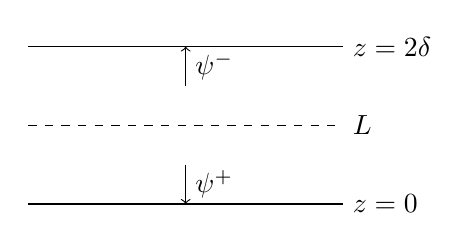
\begin{tikzpicture}
		\def\width{1.0};
		\def\length{2};
		\def\arrowLength{0.5}
		%% Draw the lines
		\draw (-{\length},{\width}) -- ({\length}, {\width});
		\draw[dashed] (-{\length}, 0) -- ({\length}, 0);
		\draw (-{\length}, -{\width}) -- ({\length}, -{\width});
		%% Draw the arrows
		\draw[->] (0, { \width -  \arrowLength }) -- (0, {\width}) 
			node[midway, right] {$\psi^-$};
		\draw[->] (0, { -\width + \arrowLength }) -- (0, {-\width})
			node[midway, right] {$\psi^+$};
		%% Label everything
		\node[right] at ({\length}, {\width}) {$\im z = 2 \delta$};
		\node[right] at ({\length}, 0) {$L$}; %{$\im z = \d$};
		% \node[left] at (-{\length}, 0) {$\psi$};
		\node[right] at ({\length}, -{\width}) {$\im z = 0$};
	\end{tikzpicture}
	\end{center}
	% \caption{Diagram representing the boundary values $\psi^\pm$.}
% \end{wrapfigure}
% \end{figure}


Using $\psi$, we define a new function $w$ by 
$w(z) = e^{-i \lambda z /2} \psi(z)$, 
where $\lambda$ is the parameter for $\mu_1$ and $\mu_2$. 
Plugging $\psi^\pm(x) = e^{\pm \delta \lambda/2} e^{i \lambda x/2} w^\pm(x)$ into 
\eqref{eq:ILW.lax.x} yields 
\begin{align*}
	i w_x^+ - \frac{\lambda}{2} w^+ + (u - \mu_1) w^+ = \mu_2 e^{-\lambda \delta} w^-
\end{align*}
which, after rearrangement, becomes
\begin{align*}
	i w^+_x + (-\lambda/2 - \mu_1) w^+ - \mu_2 e^{-\lambda \delta} w^- = - u w^+.
\end{align*}
Now
\begin{align*}
	-\lambda/2 - \mu_1 
		&= \lambda/2 \coth(\lambda \delta) - \lambda \\
		&= \frac{\lambda}{2} \(\frac{e^{\lambda \delta}+e^{-k \delta}}{e^{\lambda\delta}-e^{\lambda\delta}}-1\)\\
		&= \frac{\lambda}{2} \( \frac{2 e^{-\lambda\delta}}{e^{\lambda\delta} - e^{-\lambda \delta}} \) \\
		&= \frac{1}{2} e^{-\lambda \delta} \lambda \csch(\lambda\delta) \\
		&= e^{-\lambda \delta} \mu_2 \\
		&= \frac{\lambda}{1 - e^{-2\lambda\delta}}, 
\end{align*}
which implies
\begin{align} \label{eq:weqn}
	i w_x^+ + \zeta \( w^+ - w^- \) = - u w^+, 
\end{align}
where $\zeta:= \zeta(\lambda) = \frac{\lambda}{1 - e^{-2\lambda\delta}}$ is as defined earlier in
theses notes. Given that the steps from \eqref{eq:ILW.lax.x} to \eqref{eq:weqn} are reversible,
it follows that \eqref{eq:ILW.lax.x} and \eqref{eq:weqn} are equivalent.


Now, since
\[
	\wh w(\xi) 
		= \int_\RR e^{-i\xi x} w(x) \, \mathrm{d}x 
		= \int_\RR e^{-i\xi x} e^{i\lambda x/2} \psi(x) \, \mathrm{d}x
		= \int_\RR e^{-i(\xi - \lambda/2) x}  \psi(x) \, \mathrm{d}x
		= \wh \psi(\xi - \lambda/2),
\]
we see from the Fourier Inversion Theorem that
\begin{align}\label{eq:wFIT}
	w(x) 
		= \frac{1}{2 \pi} \int_\RR e^{i \xi x} \wh \psi(\xi - \lambda/2 ) 
			\, \mathrm{d}\xi
		= \frac{1}{2 \pi} \int_\RR e^{i \xi x} \wh w(\xi) \, \mathrm{d}\xi,
\end{align}
where we use $w(x)$ (as opposed to $w(z)$) to denote the 
restriction of $w$ to the line $L$. Thus, the boundary values for $w$.
The boundary values $w^\pm$ of $w$ are therefore given by 
\begin{align*}
	w^\pm(x) 
		= w(x \mp i \delta )
		= \frac{1}{2\pi} 
			\int_\RR e^{i\xi x} e^{\pm \delta \xi } \, \wh w(\xi) \, \mathrm{d}\xi.
\end{align*}
That is,
\begin{align*}
	w^\pm(x) = \mc F^{-1}\( e^{\pm \delta(\dotarg)} \wh w(\dotarg) \)(x),
\end{align*}
which implies 
\begin{align} \label{eq:w+w-relation}
	\wh w^+(\xi) = e^{2\delta \xi} \, \wh w^{-}(\xi).
\end{align}
% Taking $W(z) := e^{-i\lambda (z - i\delta)/2} \Psi(z)$ so that $W(z) = w(z-i\delta)$,
% we find 
We further see from \eqref{eq:wFIT} that 
\begin{align*}
	\mc F\big(w(\dotarg-i\delta + iy)\big)(\xi)
		= e^{-(y-\delta)\xi} \, \wh w(\xi)
		= e^{-y\xi} \, \wh w^+(\xi).
\end{align*}
In particular, if $\Psi(z) := w(z + i\delta)$, then
\begin{align}
	\mc F\big(\Psi( \dotarg + iy)\big)(\xi) = e^{-y\xi} \, \wh \Psi^+(\xi),
\end{align}
where $\Psi^+(x) := \lim_{y \searrow 0} \Psi(x + iy)$. Using an analogous argument for \ref{eq:ILW.lax.t}, we
rewrite \eqref{eq:ILW.lax} as
\begin{subequations}
	\label{eq:laxW}
	\begin{align}
		\label{eq:JostDE}
		L_\delta(\Psi) := \frac{1}{i} \frac{\bd}{\bd x} \Psi^+ - \zeta(\Psi^+ - \Psi^-) &= u \Psi^+ \\
		\label{eq:laxW.t}
		\frac{1}{i} \frac{\bd}{\bd t} \Psi^\pm + 2 i \( \zeta-\frac{1}{2\delta} \) + \Psi_{xx}
			&= \left[ \pm i u_x  - T u_x + \eta  \right] \Psi^\pm,
	\end{align}
\end{subequations}
where 
$
	\eta_\delta(\lambda, \delta, \nu) 
		= \lambda \( \zeta - \frac{1}{2\delta} \) + \(\frac{\lambda}{2}\)^2 + \nu,
$
and $\zeta$ can be thought of as another spectral parameter parametrized by 
$\lambda \in \mathbb R$ so that
\[
	\zeta(\lambda) = \frac{\lambda}{1- e^{-2\delta \lambda}}.
\]
Stated in another way, the ILW is an isospectral flow for the linear spectral problem 
\eqref{eq:JostDE}. 




\end{document}